\chapter{Secure Interoperation}
Si tratta della Composizione di sistemi sicuri, sistemi con attributi o politiche di sicurezza identici o compatibili che condividono dati dove c'è comunicazione quando oggetti e soggetti hanno un livello di sicurezza assegnato (sistemi multilivello). 

\begin{figure}[H]
	\centering
    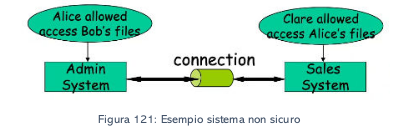
\includegraphics[width=14cm, keepaspectratio]{Bistarelli/img/secure_interoperation/int1.png}
\end{figure}

I sistemi sono individualmente sicuri.
\begin{itemize}
    \item È sicuro permettere la condivisione dei file tra i sistemi del personale e delle vendite?
    
    \begin{itemize}
        \item Clare non è autorizzata ad accedere ai file di Bob, ma Clare però può accedere ai file di Bob tramite il sistema di amministratore clare - alice - bob.
        
        \item Necessità di riconfigurare le connessioni/sistemi per chiudere questa via d'accesso tortuosa
        
        \item Nel caso sopra bisognerebbe staccare la connessione visto che Clare accede a Bob tramite Alice, perché Alice può accedere ai file di Bob.
    \end{itemize}
\end{itemize}

\begin{figure}[H]
	\centering
    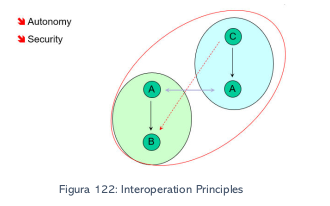
\includegraphics[width=14cm, keepaspectratio]{Bistarelli/img/secure_interoperation/int2.png}
\end{figure}

Per risolvere il problema possiamo operare su:
\begin{itemize}
    \item Interoperabilità
    
    \item Autonomia
\end{itemize}
Nel caso riportato sopra:
\begin{enumerate}
    \item \textbf{Riduzione Interoperabilità}
    
    Tolgo le relazioni I/O di 2 sistemi 
    
    \item \textbf{Riduzione di Autonomia}
    
    Tolgo l'accesso di alice ai dati di bob
\end{enumerate}

\begin{figure}[H]
	\centering
    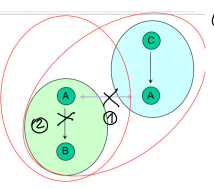
\includegraphics[width=8cm, keepaspectratio]{Bistarelli/img/secure_interoperation/int3.png}
    \caption{Sicurezza riducendo l'autonomia}
\end{figure}
Access configuration

Un insieme di vincoli tra entità (soggetti, oggetti) che specificano i permessi di accesso
\begin{itemize}
    \item Variables V = \{S,O\}
    
    \item Domain D=\{a,b,c\}
    
    \item  CS1(a,b)=T
    
    \item CS1(a,c)=F
\end{itemize}
\begin{figure}[H]
	\centering
    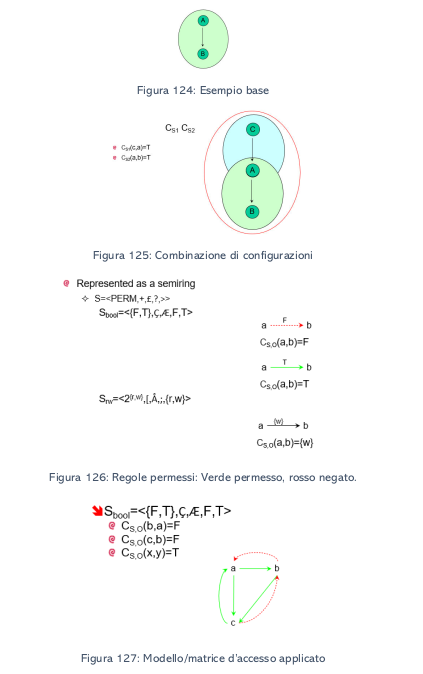
\includegraphics[width=14cm, keepaspectratio]{Bistarelli/img/secure_interoperation/int4.png}
\end{figure}
Per esempio posso non rappresentare tutti i diritti se al modello sono applicate regole di default deny o default
permitted.

\singlespacing

Se la lettera b che rappresenta l’utente fosse contenuta dentro un quadrato sarebbe transitiva, quindi
permetterebbe la transitività. Transitività quadrata - Freccia verde. Transitività tonda - Freccia rossa.

\subsection{Acces Reconfiguration}

E' necessaria per fondere 2 sistemi.

\singlespacing

Esempio fusione di due aziende con policy diverse:
\begin{itemize}
    \item se decidono di fondersi devono riconfigurare le policy in modo sicuro
    
    \item è sicuro se vengono ridotti i diritti che c’erano prima
    
    \item quindi una configurazione Cs’ è sicura se gli accessi che do sono un sottoinsieme di Cs: Gli utenti non devono avere piu' accessi di quelli che avevano prima. 
\end{itemize}
\begin{figure}[H]
	\centering
    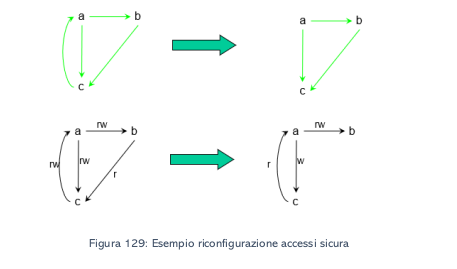
\includegraphics[width=14cm, keepaspectratio]{Bistarelli/img/secure_interoperation/int5.png}
\end{figure}
Supponiamo di avere un sistema Cs1 ed un sistema Cs3 che hanno policy e utenti diversi.
\begin{itemize}
    \item Cs1 ha gli utenti a,b,c.
    
    \item Cs3 ha gli utenti a,c,d.
\end{itemize}
\begin{figure}[H]
	\centering
    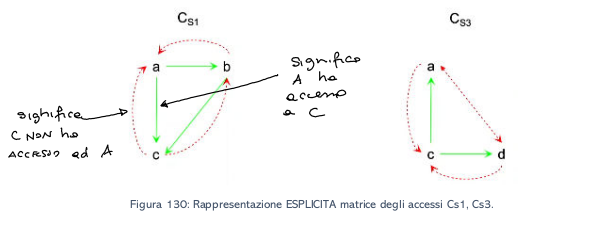
\includegraphics[width=14cm, keepaspectratio]{Bistarelli/img/secure_interoperation/int6.png}
\end{figure}
\begin{figure}[H]
	\centering
    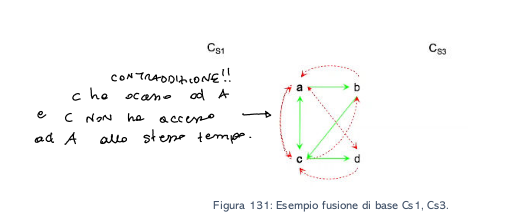
\includegraphics[width=14cm, keepaspectratio]{Bistarelli/img/secure_interoperation/int7.png}
\end{figure}
L’esempio di fusione sopra riportato non andrebbe bene, perché pieno di contraddizioni.

\singlespacing

Quindi come faccio a sapere quali sono le cose da ridurre ?

\singlespacing

Parto dalla fusione base rappresentato però solo quello che è vietato, così non ho neanche contraddizioni.

\begin{figure}[H]
	\centering
    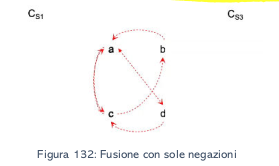
\includegraphics[width=11cm, keepaspectratio]{Bistarelli/img/secure_interoperation/int8.png}
\end{figure}

Quindi, proseguo aggiungendo i verdi (Indicano che ho l'accesso) per Cs1 e Cs3 dove non ci sono contraddizioni:

\begin{figure}[H]
	\centering
    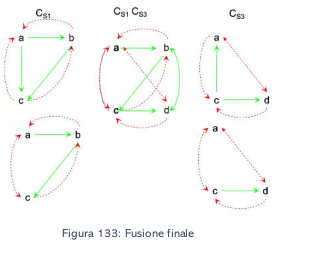
\includegraphics[width=14cm, keepaspectratio]{Bistarelli/img/secure_interoperation/int9.png}
\end{figure}

Essendo C transitiva, A non può accedere a B perché A non accedere a C e C non può accedere a B. Stessa
cosa per D e B. Aggiungo quindi più frecce rosse rispetto a sistemi non transitivi e non aggiungerò frecce verdi
dove è presente la proprietà transitiva.

\begin{figure}[H]
	\centering
    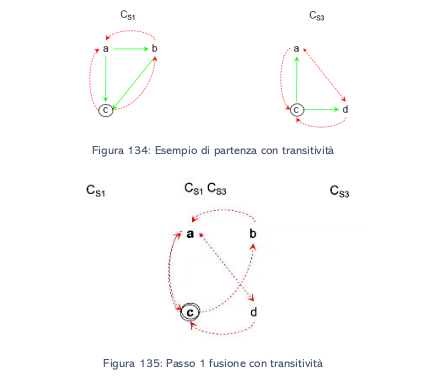
\includegraphics[width=14cm, keepaspectratio]{Bistarelli/img/secure_interoperation/int10.png}
\end{figure}

Proietto Cs1 e Cs3 su  Cs1 e Cs3, solo gli archi su cui non abbiamo contraddizioni 
\subsection{Acces Transitivity}

\begin{figure}[H]
	\centering
    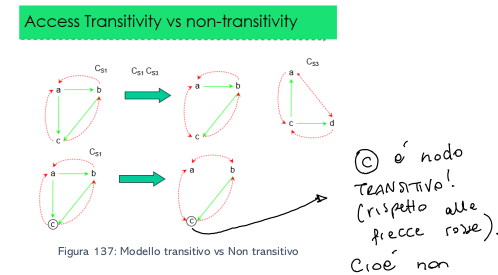
\includegraphics[width=14cm, keepaspectratio]{Bistarelli/img/secure_interoperation/int11.png}
\end{figure}

Le strategie principali per una massimale rinconfigurazione di sistema sono 2:
\begin{enumerate}
    \item Rimuovere il numero minimo degli archi
    
    \item Ridurre il numero degli archi mantenendo il massimo delle connessioni
\end{enumerate}
Esempio riconfigurazione:
\begin{itemize}
    \item Sistema 1: Arco verde A - B
    
    \item Sistema 2: Arco verde B - C
    
    \item B transitivo, quindi A - C
    
    \item  Se però nella fusione mi ritrovo una policy con arco rosso tra A e C devo riconfigurare in modo diverso i sistemi. Avrei tre opzioni:
    
    \begin{itemize}
        \item Togliere la freccia da A a B sul sistema 1
        
        \item Togliere la freccia da B a C sul sistema 2
        
        \item Elimino la transitività di B
    \end{itemize}
\end{itemize}

\begin{figure}[H]
	\centering
    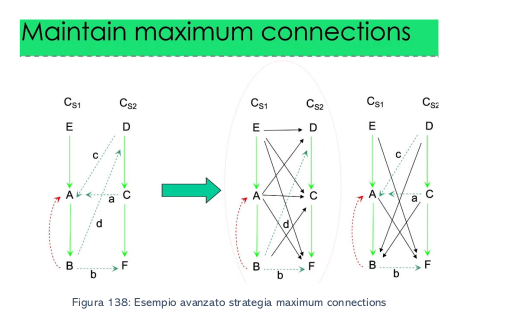
\includegraphics[width=14cm, keepaspectratio]{Bistarelli/img/secure_interoperation/int12.png}
\end{figure}

Topologie speciali:
\begin{itemize}
    \item Forma ad albero (sistema master e interoperabilità locale)
    
    \begin{itemize}
        \item Tempo polinomiale
    \end{itemize}
    
    \item Vita reale:
    
    \begin{itemize}
        \item Client-server vs Peer-to-peer
    \end{itemize}
\end{itemize}
\subsection{Sistemi speciali: multilevel security}
Considera il rischio di assurance nella composizione di sistemi sicuri multilivello valutati in base a criteri di
valutazione della sicurezza.
\begin{itemize}
    \item L'analisi della sicurezza di sistemi interoperanti e individualmente sicuri può essere fatta in tempo polinomiale.
    
    \item Data una configurazione di rete non sicura, allora riconfigurare le connessioni in modo ottimale (per minimizzare l'impatto sull'interoperabilità) è NP.
\end{itemize}
Esempio sistema MLS:
\begin{itemize}
    \item A è in grado di gestire informazioni di 2 categorie: Secret e top secret
    
    \item N è in grado di gestire informazioni di 3 categorie: Secret, top secret e unclassified
    
    \item C è in grado di gestire informazioni di 2 categorie: Secret e unclassified
    
    \item Quale dovrebbe essere configurata in modo più stringente? La B perché ha più livelli di informazione (3) rispetto ad A e C e perchè un attaccante ha più livelli da attaccare. Avendo più livelli un sistema in genere più affidabile.
\end{itemize}

\begin{figure}[H]
	\centering
    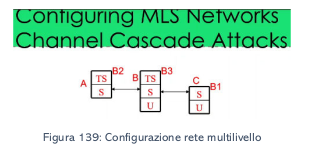
\includegraphics[width=14cm, keepaspectratio]{Bistarelli/img/secure_interoperation/int13.png}
\end{figure}

Nella figura TS non deve essere collegato a S visto che hanno un livello diverso di sicurezza. Le frecce in
genere sono bidirezionali.

\singlespacing

Gli evalutation criteria sono livelli di assurance che indicano quanto ci si può fidare di una macchine (testo di
riferimento citato a lezione: orange book, sicurezza multilivelli. | red book per le connessioni tra questi livelli di
sicurezza).

\singlespacing

Ogni macchina ha un livello di assurance a seconda dei livelli confidenzialità delle informazioni che gestiscono.

\singlespacing

Multilevel security modello Bell LaPadula:
\begin{itemize}
    \item Livelli di sicurezza L definiscono la classificazione dei soggetti (processi) e degli oggetti.
    
    \begin{itemize}
        \item Per esempio, Non classificato, Segreto, Top-Secret.
    \end{itemize}
    
    \item Politica: reticolo di livelli di sicurezza $(L,<=)$
    
     \begin{itemize}
        \item $x<=y:$ le informazioni del livello x possono passare al livello y.
        
        \item Non classificato $<$ Segreto $<$ Top-Secret
    \end{itemize}
\end{itemize}
Per l’esempio riportato nella figura sopra si utilizza la logica di Bell LaPadula per la gestione e la comunicazione
tra livelli.

\singlespacing

Evaluation Criteria ["Orange" e "Red" Books]
\begin{itemize}
    \item Sistemi MLS assicurati a diversi livelli di garanzia basati su criteri di valutazione.
    
    \begin{itemize}
        \item (peggiore) $D<C1<C2<C3<B1<B2<B3<A1$ (migliore).
        
        \item I sistemi valutati devono soddisfare i requisiti minimi di rischio.
        
        \item I sistemi che memorizzano combinazioni di dati ad alto rischio hanno bisogno di alti livelli di garanzia
    \end{itemize}
\end{itemize}

\begin{figure}[H]
	\centering
    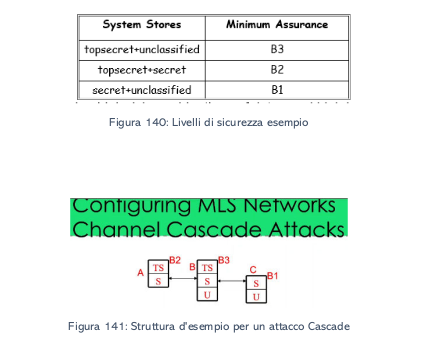
\includegraphics[width=14cm, keepaspectratio]{Bistarelli/img/secure_interoperation/int14.png}
\end{figure}

Esempi attacchi Cascade

\begin{itemize}
    \item Supponiamo che i singoli sistemi A, B, C sono sicuri.
    
    \item Ogni sistema valutato soddisfa i criteri.
    
    \item  Tuttavia, la rete ha un rischio a cascata:
    
    \begin{itemize}
        \item L'attaccante rompe il sistema A, copia i dati TS a S
        
        \item Copia questi dati dal sistema A a B a C
        
        \item Rompe il sistema C, copia i dati di S(TS) in U.
        
        \item L’assurance B3 è richiesta quando si proteggono TS e U, ma un attacco a cascata rompe i sistemi B2 e inferiori.
    \end{itemize}
\end{itemize}

\begin{figure}[H]
	\centering
    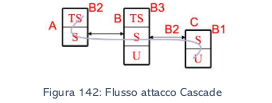
\includegraphics[width=14cm, keepaspectratio]{Bistarelli/img/secure_interoperation/int15.png}
\end{figure}

Usando questa strategia si evita lo sforzo di livello 3 per ‘rompere’ B3.
\\
In questo caso ho uno sforzo di livello 2 andando inizialmente su B2, poi successivamente porto l’informazione
da TS ad U sul sistema C che è anch’esso uno sforzo di livello 2. Con questo Cascade Path l’effort/sforzo è
minore del costo dell’attacco perché costa 2 invece di 3, quindi si dice che uno sforzo 2 per un
guadagno 3. Andando direttamente a rompere B3 invece mi sarebbe costato 3 e non ci sarebbe stato un attacco
Cascade. In conclusione per passare da TS ad U uso B2 e B1 (passando per B3) e non B2 per poi andare a
rompere B3, perché costerebbe di più.

\begin{figure}[H]
	\centering
    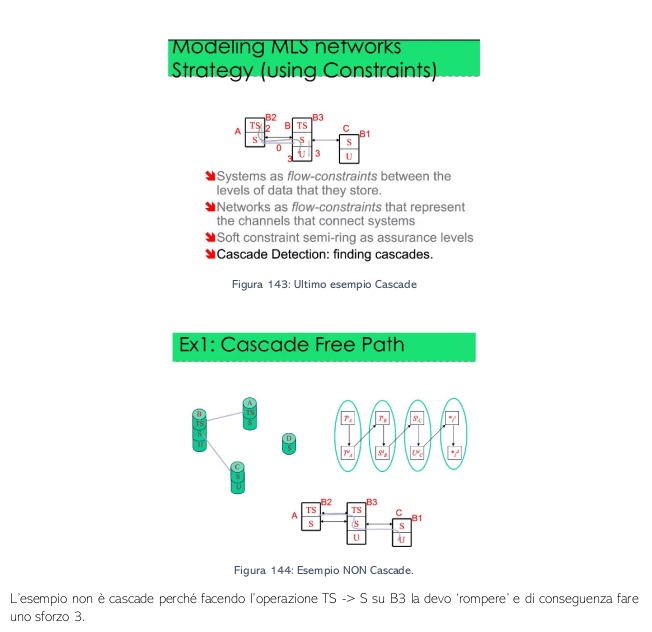
\includegraphics[width=14cm, keepaspectratio]{Bistarelli/img/secure_interoperation/int16.png}
\end{figure}
